
\label{chap:th_model_vr_1}
%\section{Motivace}
%\label{sec:the_model_vr_1_motivace}
Studium přirozené konvekce na školním reaktoru VR-1 je klíčové pro zajištění bezpečného provozu tohoto zařízení. Při studiu nucené konvekce je průtok sledovaným objemem určen jako vstupní parametr, resp. jako okrajová podmínka. Pro přirozenou konvekci není průtok vstupním parametrem, ale je odvozen z teplotního gradientu a je dáno modelem samotného reaktoru. U výzkumných reaktorů bazénového typu (např. VR-1, TRIGA Mark II) musí být model reaktoru rozšířen o reaktorovou nádobu, aby bylo možné odhadnout celkový průtok skrze zónu \cite{TRIGA_CFD}. Cílem této kapitoly je popis termohydraulického modelu školního reaktoru VR-1 a studium vlivu nodalizace obtoku na přirozené proudění.

Na obr. \ref{fig:cfd_triga_reynolds} je pomocí CFD kódu uvedena Reynoldsova mapa, resp. rychlostní pole v případě přirozeného proudění skrze AZ reaktoru TRIGA Mark II (geometrie reaktoru TRIGA je zobrazena v příloze na obr. \ref{fig:triga_geometrie}). Reaktor TRIGA Mark II a školní reaktor VR-1 mají obdobnou konstrukci a oba jsou bazénového typu (viz obrázek \ref{fig:vr_1_geometrie} v příloze). Z obrázků \ref{fig:cfd_triga_reynolds} a \ref{fig:cfd_triga_velocities} vyplývá, že nejvíce turbulentní proudění nastává v prostoru nad aktivní zónou, tedy i v horní části vertikálního obtoku skrz reaktorovou nádobu. Obrázek \ref{fig:cfd_triga_velocities} naznačuje, že změna teplotního gradientu nad aktivní zónou vede k vzniku inverze proudění a tvorbě smyček. Z tohoto důvodu se tato kapitola soustředí především na studium této oblasti (viz obrázek \ref{fig:nod_00}). Dále je oblast volného objemu nad aktivní zónou označena jako "horizontální obtok" a komponenta 44 jako "vertikální obtok".



\begin{figure}[H]
	\centering
	\begin{subfigure}{0.5\textwidth}
		\centering
		\vspace{0cm}
		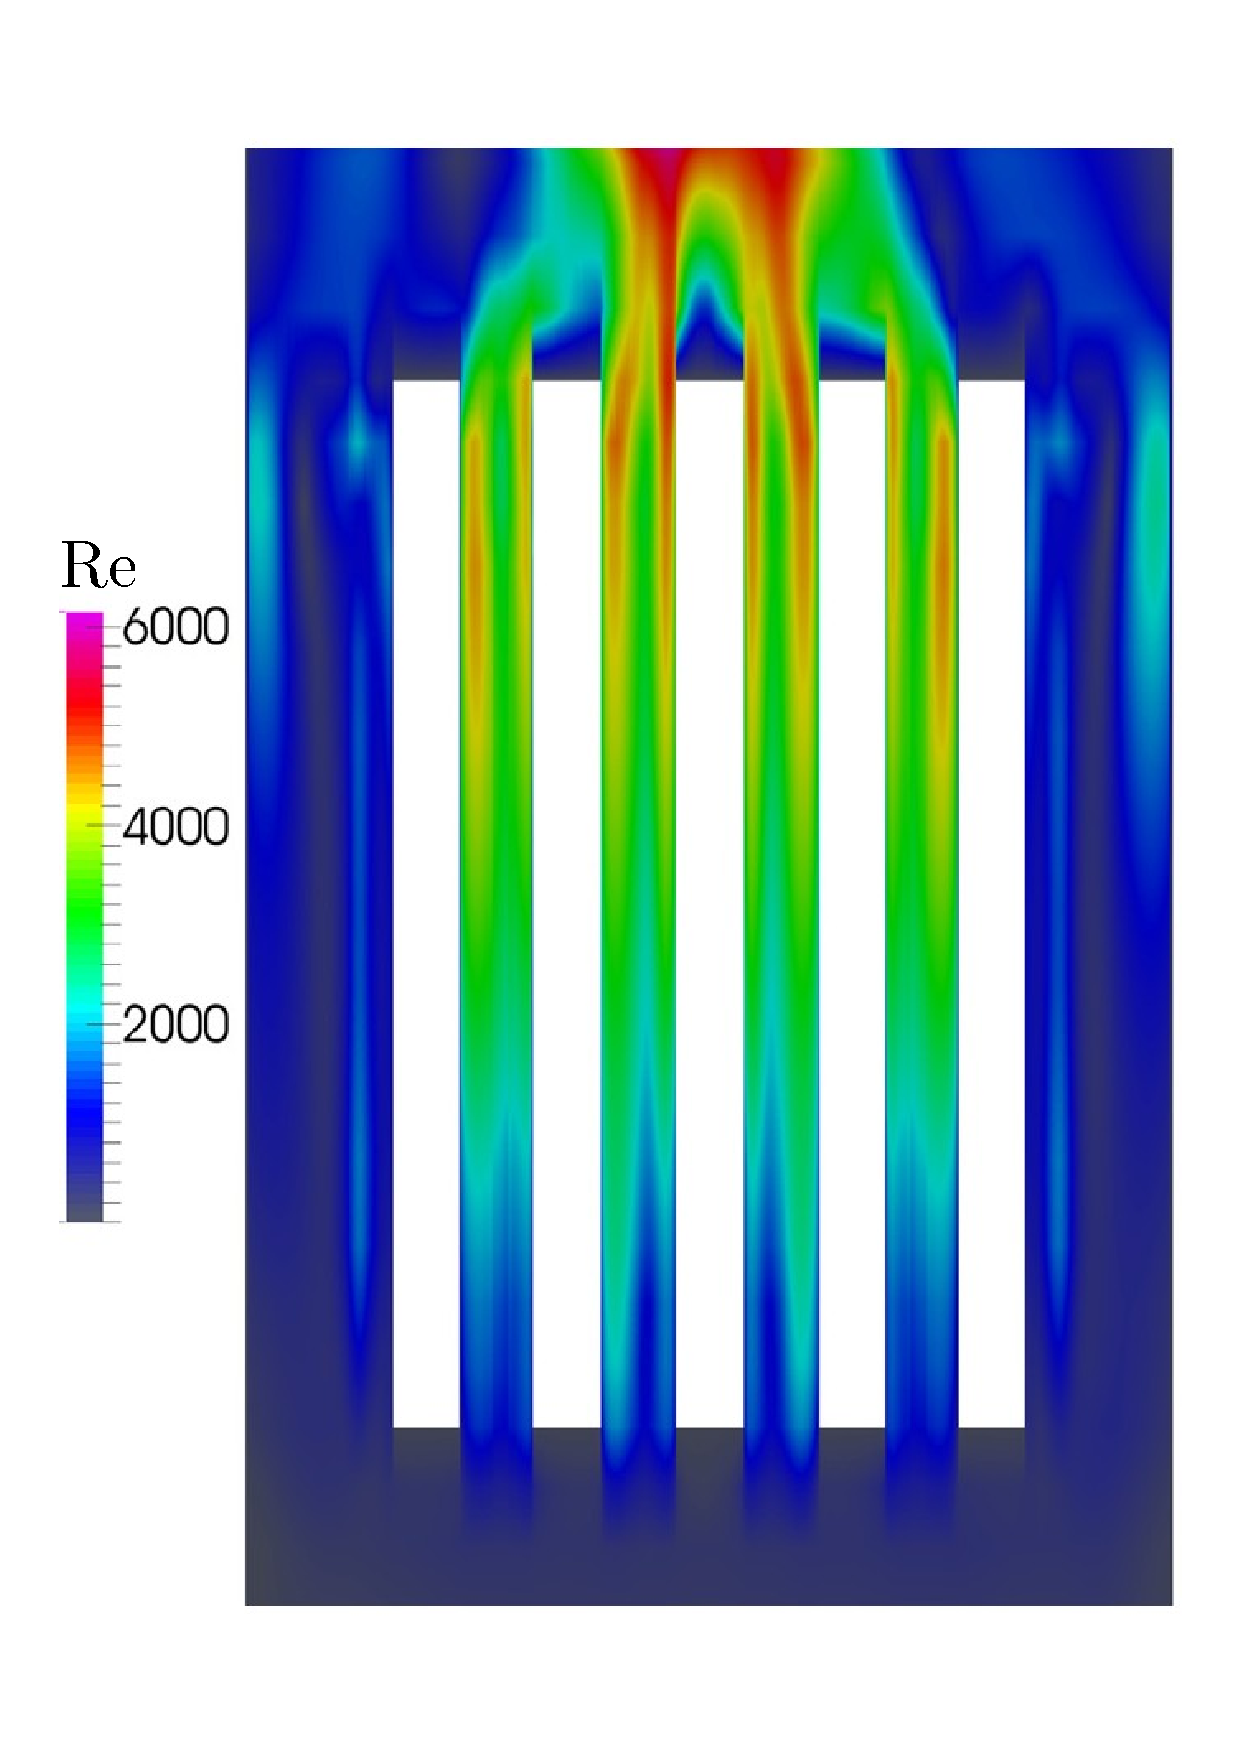
\includegraphics[width=0.6\textwidth, trim={1cm 2cm 1cm 2cm}, clip]{./05_TH_model_VR_1/obrazky/cfd_triga_reynolds_number.pdf}
		\vspace{0pt}
			\caption{Reynoldsova mapa}
			\label{fig:cfd_triga_reynolds}
	\end{subfigure}%
	\hfill
	\begin{subfigure}{0.5\textwidth}
		\centering
		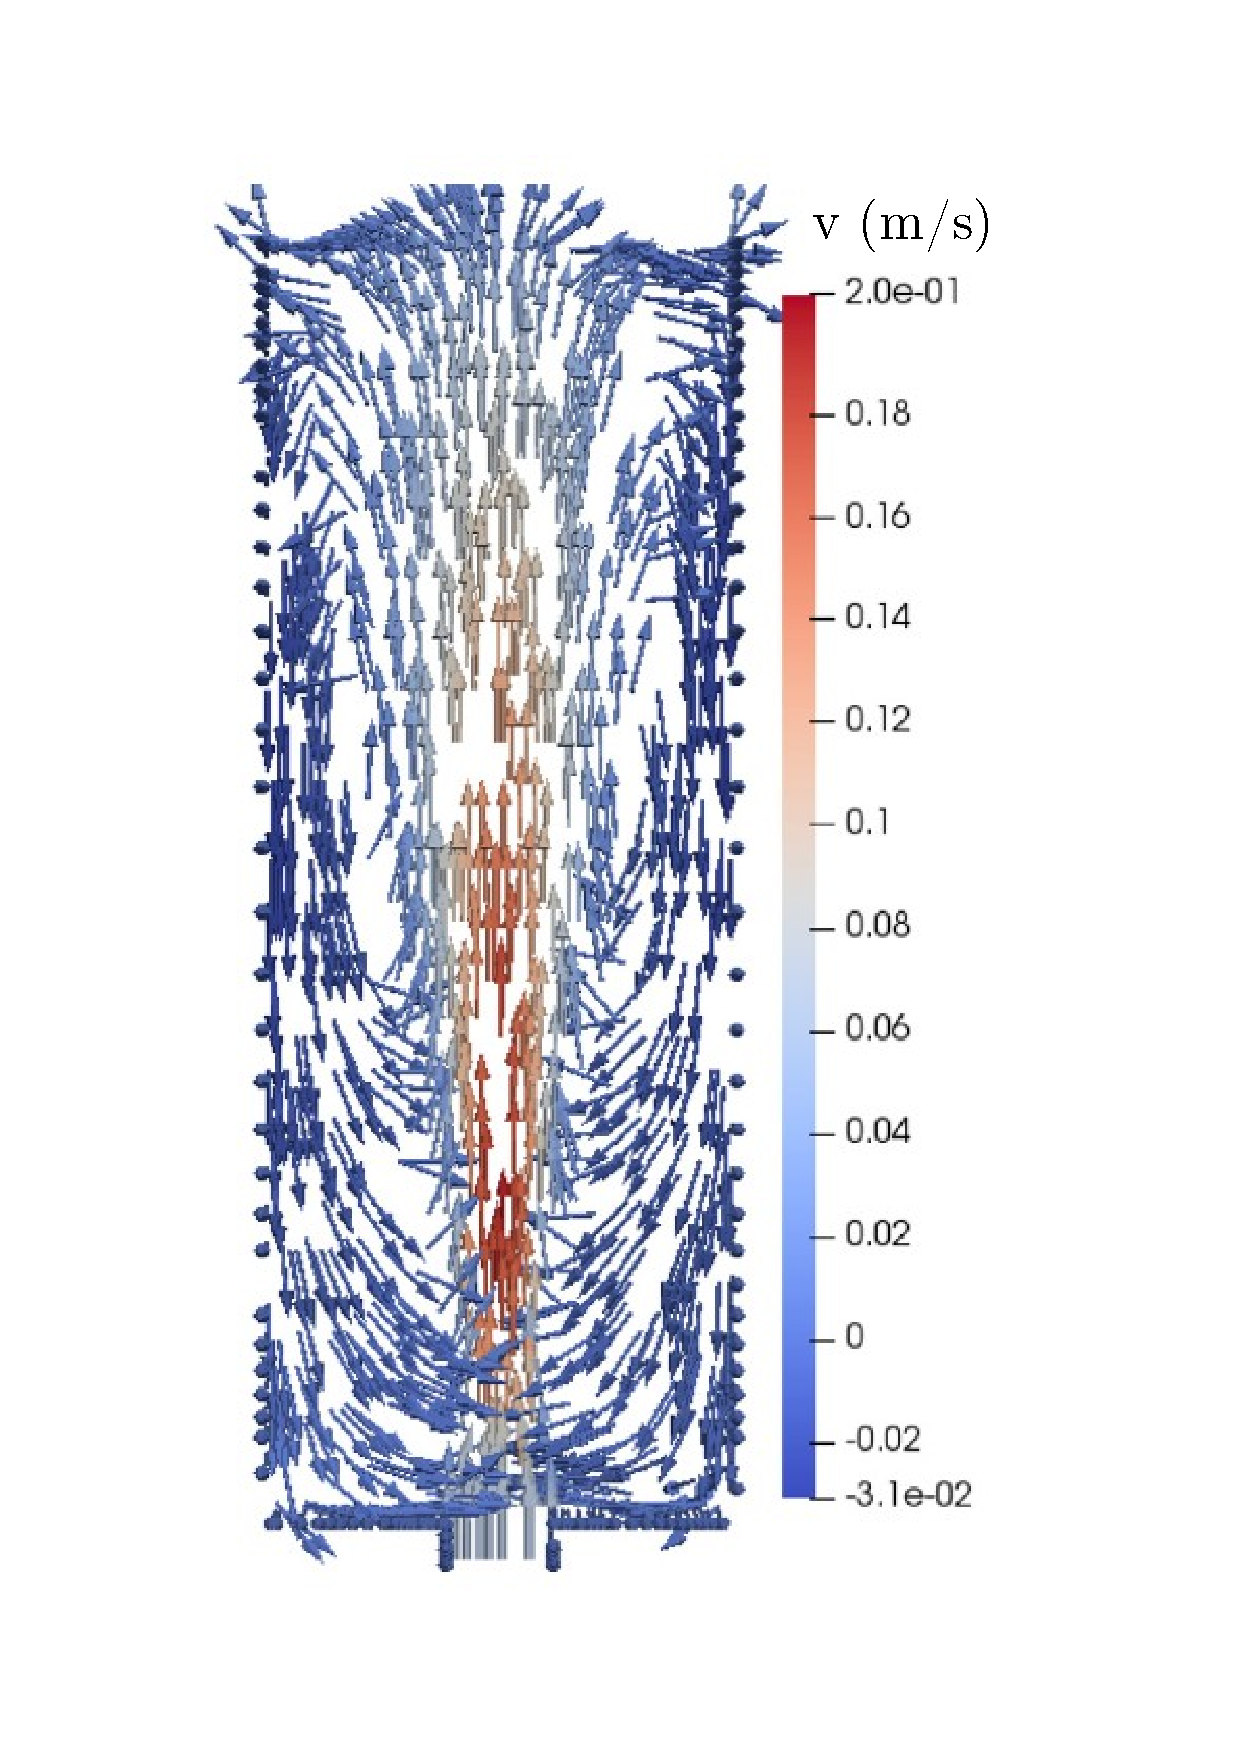
\includegraphics[width=0.6\textwidth, trim={2cm, 3cm, 2cm, 3cm}, clip]{./05_TH_model_VR_1/obrazky/triga_cfd_velocities.pdf}
		\caption{Rychlostní pole}
		\label{fig:cfd_triga_velocities}
	\end{subfigure}
	\caption{CFD výpočet přirozeného proudění skrze reaktor TRIGA MARK II \cite{TRIGA_CFD}.}
\end{figure}


\section{Referenční model}
\label{sec:referencni_model}
V této práci \cite{fejt} byl při tvorbě modelu školního reaktoru VR-1 opuštěn koncept dvoukanálového uspořádání, který využíval "průměrný" a "maximální" kanál pro reprezentaci aktivní zóny reaktoru. Místo toho byla aktivní zóna sestavena z 16 palivových článků (PČ), z nichž každý byl reprezentován jednotkovým modelem (viz sekce \ref{sec:sjednoceni_topnych_komponent}). Kvůli omezenému počtu připojitelných komponent k jednotce BRANCH (komponenta 100 a 102) byla aktivní zóna reprezentována dvěma skupinami po osmi PČ, které byly propojeny spojovací jednotkou. Všechny jednotkové modely vychází z modelu 8-trubkového PČ bez vytěsnitele, přičemž axiální rozložení výkonu jednotlivých PČ odpovídá tabulce \ref{tab:rozlozeni_vykonu_irt_serpent}. Geometrie trubek horizontálního a vertikálního obtoku je stejná jako v modelu, který je popsán na obrázcích \ref{fig:irt_nat_conv_komplex} a \ref{fig:irt_nat_conv_jedno}. Zapojení komponent 40-48 vychází z práce \cite{fejt}. Model na obrázku \ref{fig:nod_00} je označen jako "referenční", resp. jako model NOD00. Nodalizace reaktoru bude podrobněji rozebrána v následujících kapitolách.

V případě referenčního modelu je horizontální obtok napojen až v posledním nódu trubky 40. Voda je vytlačena z AZ až na úroveň hladiny, kde se odpojuje do horizontálního obtoku. V tomto uspořádání je teplotní gradient mezi výstupem z AZ reaktoru a TDV 50 představující volnou hladinu největší (tlak \SI{1,5e5}{\pascal} Pa a teplota vody 297 K). Nikde v trubce 40 nedochází k ochlazení bočním vtokem. U referenčního modelu je proto očekáván nejvyšší průtok.

Výkon školního reaktoru VR-1 je pro studium přirozeného proudění příliš nízký (\SI{1e2}{\watt}, nárazově \SI{5e2}{\watt}). Proto je v následujícím textu uvažován výkon jednoho PČ \SI{1e4}{W} (celkový výkon AZ \SI{1,6e5}{\watt}), při kterém je studium přirozené konvekce názornější. Stále se jedná o jednofázové proudění podchlazené kapaliny. Průběh výkonu jednotkového modelu PČ je uveden v příloze v Tab. \ref{tab:vykon_model} (více o jednotkovém modelu v sekci \ref{sec:sjednoceni_topnych_komponent}). Aktivní zóna je tvořena 16 PČ, každý článek má výkon \SI{10e4}{\watt}. Celkový výkon reaktoru dosahuje v čase 20 s \SI{1,6e5}{\watt}. Na obr. \ref{fig:temp_fuel_nod00} je uvedeno rozdělení teplot chladiva v PČ v čase 10 s, 20 s, 30 s a 40 s po dosažení výkonu \SI{10e4}{\watt}. Celkový průtok PČ je uveden na obr. \ref{fig:nod_00_mass_flow_rate}.
\subsection{Výsledky}

 
\begin{figure}
	\centering
	\includegraphics[width=\textwidth, trim={1cm 218cm 148cm 5cm}, clip]{./06_hodnoceni_TH_modelu/obrazky/nod_00_recirculation.pdf}
	\caption{Termohydraulický model reaktoru VR-1.}
	\label{fig:nod_00}
\end{figure}


\begin{figure}[H]
	\centering
	\begin{subfigure}{0.5\textwidth}
		\centering
		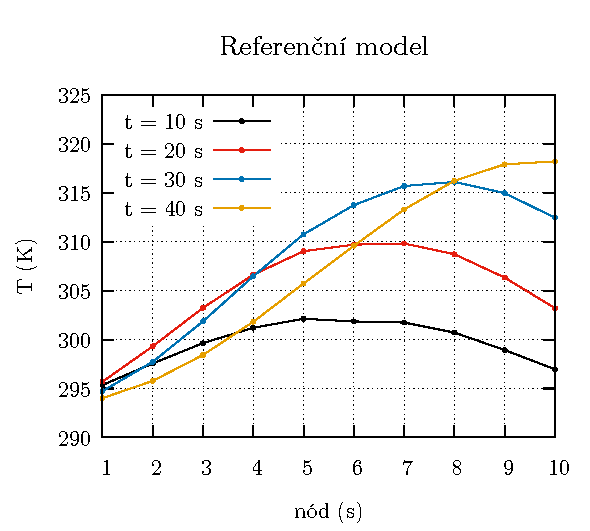
\includegraphics[width=\textwidth, trim={0cm 0cm 0cm 0cm}, clip]{./05_TH_model_VR_1/grafy/nod_00_temp_distribution_fuel.pdf}
		\caption{Axiální rozložení teplot vody v PČ.}
		\label{fig:temp_fuel_nod00}
	\end{subfigure}%
	\hfill
	\begin{subfigure}{0.5\textwidth}
		\centering
		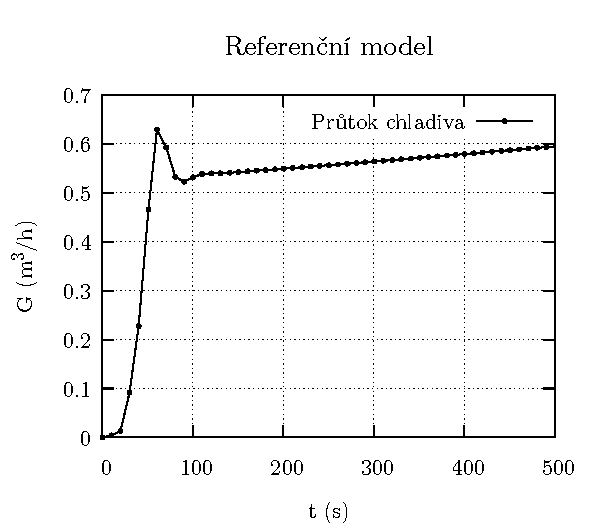
\includegraphics[width=\textwidth, trim={0cm 0cm 0cm 0cm}, clip]{./05_TH_model_VR_1/grafy/nod_00_mass_flow_rate_fuel.pdf}
		\caption{Celkový průtok skrze PČ.}
		\label{fig:nod_00_mass_flow_rate}
	\end{subfigure}
	\caption{Popis přirozeného proudění skrze palivový článek pro referenční model.}
\end{figure}
Na obr. \ref{fig:temp_fuel_nod00} a \ref{fig:nod_00_mass_flow_rate} lze pozorovat vznik přirozeného proudění chladiva v palivovém článku (PČ) v závislosti na čase a výkonu. Po dosažení výkonu $10^4$ W v čase 10 s je rozložení teplot symetrické, což odpovídá symetrii výkonu po axiální ose. V dalších časových krocích se teplotní maximum posouvá zhruba o 1 nód za 10 s v důsledku vzniku přirozené konvekce. Proudění ohřívaného objemu vede ke snížení teploty v dolní části palivového článku vlivem promíchávání se vstupujícím chladivem.

Na stejném obrázku je také vykreslen časový průběh průtoku chladiva skrze PČ. Vliv časového zpoždění je zde také pozorovatelný. V čase 0-60 s dochází k nárůstu průtoku v důsledku ohřevu chladiva v AZ reaktoru. Vyšší průtok v tomto případě způsobuje lepší přestup tepla a tedy i nižší teplotní gradient mezi AZ a vstupem do horizontálního obtoku, což vede ke snížení průtoku až do času 90 s. Následně se průtok ustálí okolo 100 s a hodnota průtoku lineárně roste. Důvodem je absence teplotních ztrát v modelu.

Na obrázku \ref{fig:nod_00_temp_pipe_40} jsou zobrazeny teploty v trubce 40 pro jednotlivé nódy. Teplota v nódu 1 se po 800 s ustálí, přičemž dochází k postupnému ohřevu výše položených nódů. Jelikož model neuvažuje tepelné ztráty, tak není jisté jak by vypadalo rozložení teplot době delší než 1200 s. Fyzikální význam by byl diskutabilní. Podrobnější rozložení teplot je popsáno v příloze na obrázcích \ref{fig:temp_dist_srovnani_prilohy_100s} až \ref{fig:temp_dist_srovnani_prilohy_600s}.




 
 \begin{figure}[H]
 	\centering
 	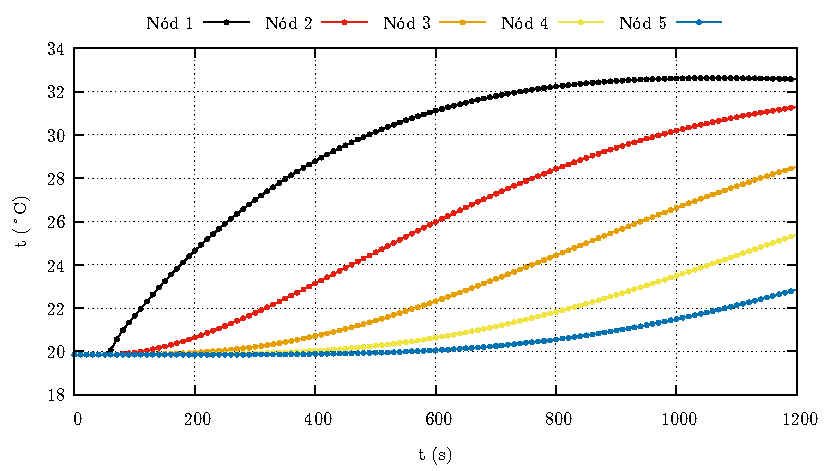
\includegraphics[width=0.8\textwidth]{./05_TH_model_VR_1/grafy/t_nod_00.pdf}
 	\caption{Časový vývoj teplot v jednotlivých nódech trubky 40.}
 	\label{fig:nod_00_temp_pipe_40}
 \end{figure}
 \section{Model NOD01}
 \label{sec:nod_01}
V referenčním modelu reaktoru VR-1 v programu RELAP5 je při simulaci přirozeného proudění předpokládána absence recirkulace ve volném objemu nad AZ, neboť je v tomto případě ohřátá voda nucena proudit až na úroveň vodní hladiny, kde se dochází k vstupu do horizontálního obtoku z posledního nódu trubky 40. Ve skutečnosti však může při přirozeném proudění docházet k odpojení vody v libovolné výšce objemu vytyčeného nad aktivní zónou. Z tohoto důvodu je trubka 42 nahrazena pěti horizontálními trubkami (trubka 170-174) viz obr. \ref{fig:nod_01}, přičemž celkový objem těchto trubek je zachován. Kompletní model je prezentován na obr. \ref{fig:nod_01_prilohy} v příloze.

  
 \begin{figure}[H]
 	\centering
 	\includegraphics[width=0.8\textwidth,  trim={7.5cm 243cm 155cm 5cm}, clip]{./07_prilohy/recirkulace/nod_01_recirculation.pdf}
 	\caption{Nodalizace horizontálního obtoku - model NOD01}
 	\label{fig:nod_01}
 \end{figure}
\subsection{Výsledky}
Z předchozího textu vyplývá, že hlavními sledovanými parametry pro srovnání referenčního a renodalizovaného modelu jsou celkový průtok skrze aktivní zónu, průtok skrze jednotlivé trubky horizontálního obtoku a rozložení teplot chladiva v trubce 40.

Renodalizovaný model NOD01 prokazuje identické chování jako referenční model v intervalu 0-200 s. Po ustálení průtoku je hodnota G(t) pro model NOD01 v čase konstantní, zatímco v referenčním modelu roste s konstantní rychlostí. Při pozorování horizontálního obtoku se ukazuje, že na rozdíl od referenčního modelu dochází k inverzi proudění v trubkách 170 a 171. Ohřáté chladivo teče vzhůru a v horizontálním kladném směru proudí trubkou 172, 173 a 174 do trubky 175, kde dochází k promíchávání. Část chladiva se následně vrací trubkou 170 a 171, kde v trubce 40 ochlazuje chladivo vystupující z AZ. Situace je ilustrována na Obr. \ref{fig:nod_01}.

Toto promíchání chladiva s ochlazenou kapalinou vstupující z trubek 170 a 171 má vliv na rozložení teplot v objemu trubky 40 viz příloha obr. \ref{fig:temp_dist_srovnani_prilohy_100s} až \ref{fig:temp_dist_srovnani_prilohy_600s}. Renodalizovaný model NOD01 tak více odpovídá reálné situaci. Je třeba zmínit, že model NOD01 neobsahuje tepelné ztráty, což má za následek konstantní nárůst teploty. Otázkou zůstává, do jaké míry je možné tento ohřev považovat za reprezentativní. 




 \begin{figure}[H]
 	\centering
 	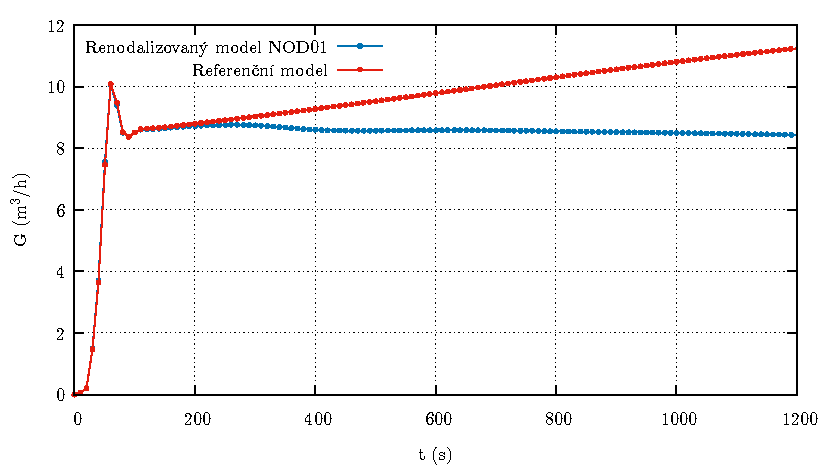
\includegraphics[width=0.8\textwidth]{./05_TH_model_VR_1/grafy/nod_01_mass_flow_rate_vertical.pdf}
 	\caption{Průtok skrze AZ reaktoru VR-1 - referenční a renodalizovaný model NOD01. }
 	\label{fig:nod_01_mass_flow_rate_vertical}
 \end{figure}
\begin{figure}[H]
	\centering
	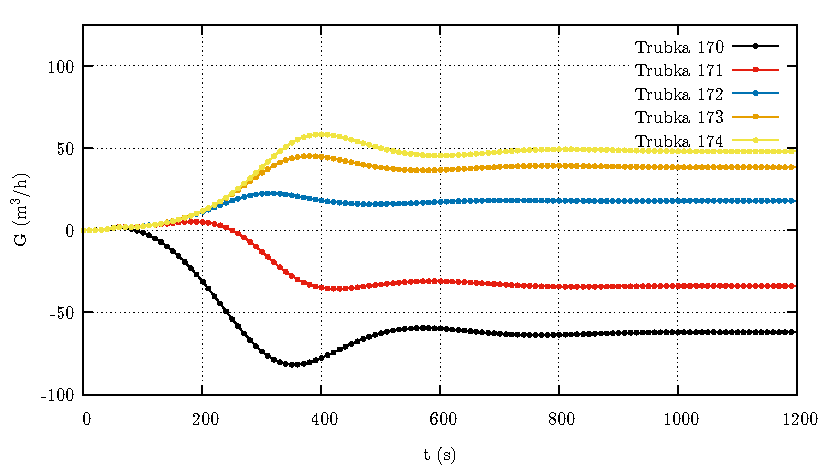
\includegraphics[width=0.8\textwidth]{./05_TH_model_VR_1/grafy/nod_01_mass_flow_rate_horizontal.pdf}
	\caption{Průtok skrze trubky 170 - 174 (viz obr. \ref{fig:nod_01}) - renodalizovaný model NOD01.}
	\label{fig:nod_01_mass_flow_rate_horizontal}
\end{figure}
\begin{figure}[H]
	\centering
	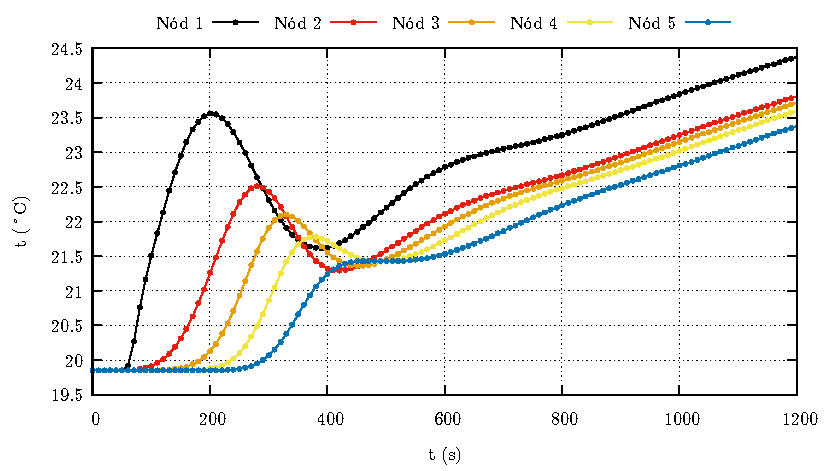
\includegraphics[width=0.8\textwidth]{./05_TH_model_VR_1/grafy/t_nod_01.pdf}
	\caption{Teplotní vývoj v trubce 40 - model NOD01.}
	\label{fig:nod_01_temp_pipe_40}
\end{figure}
%\begin{figure}[H]
%	\centering
%	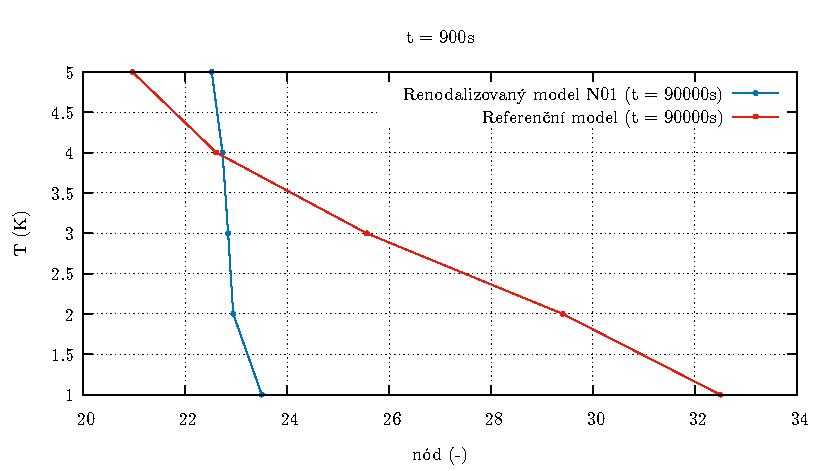
\includegraphics[width=0.8\textwidth]{./05_TH_model_VR_1/grafy/nod_01_900.pdf}
%	\caption{Distribuce teplot v trubce 40 v čase 900 s.}
%	\label{fig:nod_01_temp_distribution}
%\end{figure}
 \section{Model NOD02}
 \label{sec:nod_02}
 Druhý renodalizovaný model s označením NOD02 je konstruován za účelem studia vlivu nodalizace vertikálního obtoku. Konstrukce vertikálního obtoku i s výslednými směry proudění je ilustrována na obrázku \ref{fig:nod_02} a kompletní schéma modelu je uvedeno na obr. \ref{fig:nod_02_prilohy} v příloze. Vertikální obtok je sestaven symetricky, přičemž celkový objem trubek a kontrolních objemů je zachován. Trubka 44 v referenčním modelu je nahrazena párem propojených trubek s označením 169 a 171, které umožňují vzniku příčného proudění a redistribuci průtoku ve vertikálním směru v obou trubkách.
 \begin{figure}[h]
 	\centering
 	\includegraphics[width=0.6\textwidth,  trim={18cm 225cm 152cm 10cm}, clip]{./07_prilohy/recirkulace/nod_02_recirculation.pdf}
 	\caption{Nodalizace vertikálního obtoku - model NOD02}
 	\label{fig:nod_02}
 \end{figure}
\subsection{Výsledky}
Průtok skrze aktivní zónu reaktoru je v případě modelu NOD02 totožný s referenčním viz obr. \ref{fig:nod_02_mass_flow_rate_vertical}. Teplota v kontrolním objemu 167 je 293 K (teplota okrajové podmínky stanovené TDV 50 viz příloha obr. \ref{fig:nod_02_prilohy}). Je možné dále očekávat rozdílný průtok v obou směrech skrze SJ 178 až 185, a to z důvodu asymetrickému propojení s horizontálním obtokem. Průtok ve vertikálním obtoku je ilustrován na obrázcích \ref{fig:nod_02_mass_flow_rate_horizontal} a \ref{fig:nod_02_mass_flow_rate_vertical}. Průtok jednotlivými SJ mezi trubkou 169 a 171 se po ustálení drží konstantní hodnoty. V čase okolo \SI{1e3}{s} ovšem dochází k náhlé redistribuci průtoku. Obrázek \ref{fig:nod_02_mass_flow_rate_horizontal} naznačuje, že změnu v proudění v čase okolo 1000 s by mohlo způsobit ohřáté chladivo proudící z AZ do vrchní části vertikálního obtoku. Ani model NOD02 neobsahuje tepelné ztráty, což může způsobit nestabilní chování. 
\begin{figure}[H]
	\centering
	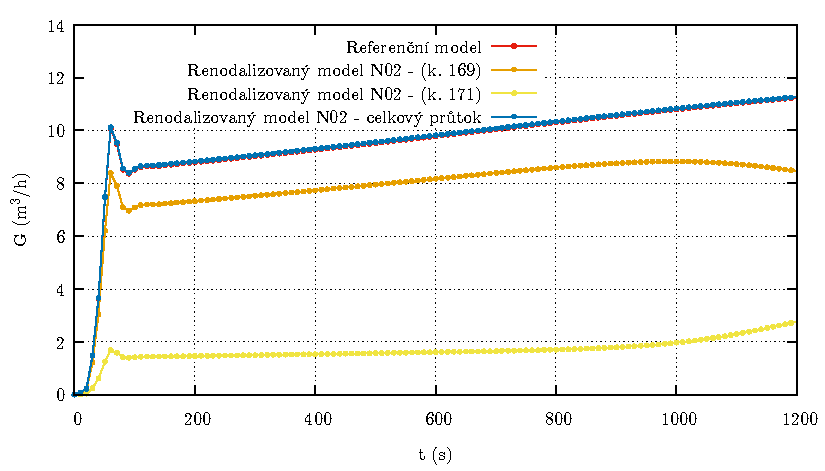
\includegraphics[width=.8\textwidth]{./05_TH_model_VR_1/grafy/nod_02_mass_flow_rate_vertical}
	\caption{Průtok skrze AZ reaktoru VR-1 - referenční a renodalizovaný model NOD02.}
	\label{fig:nod_02_mass_flow_rate_vertical}
\end{figure}
\begin{figure}[H]
	\centering
	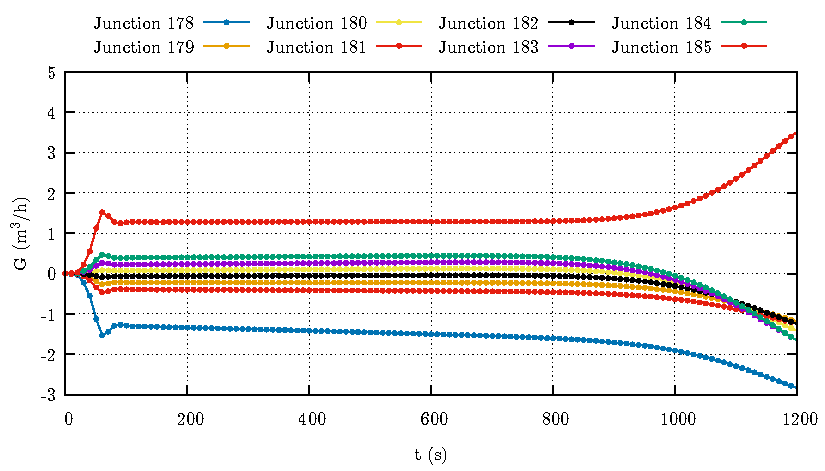
\includegraphics[width=0.8\textwidth]{./05_TH_model_VR_1/grafy/nod_02_mass_flow_rate_horizontal.pdf}
	\caption{Průtok spojovacími jednotkami (SJ) ve vertikálním obtoku - model NOD02.}
	\label{fig:nod_02_mass_flow_rate_horizontal}
\end{figure}
%\begin{figure}[H]
%	\centering
%	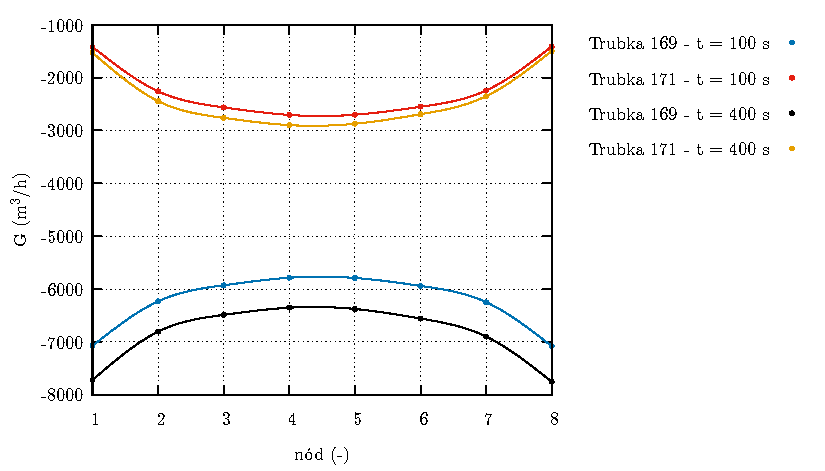
\includegraphics[width=0.8\textwidth]{./05_TH_model_VR_1/grafy/nod_02_vertikal_obtok.pdf}
%	\caption{Průtok v jednotlivých nódech trubek 169 a 171.}
%	\label{fig:nod_02_vertikal_obtok}
%\end{figure}
\begin{figure}[H]
	\centering
	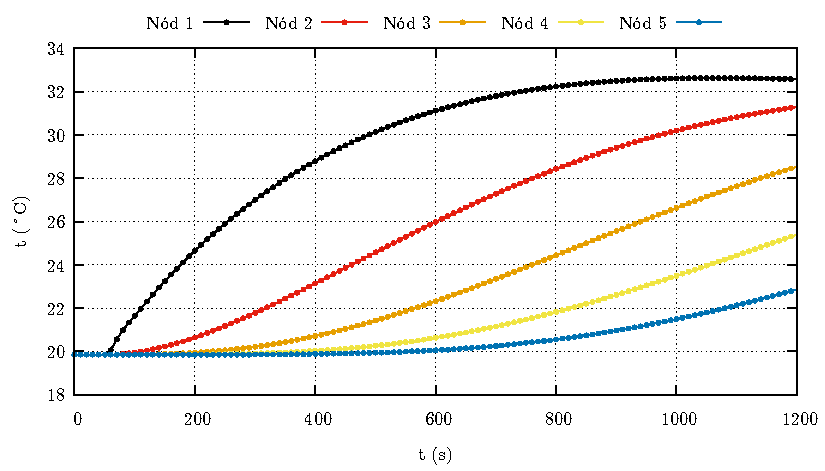
\includegraphics[width=0.8\textwidth]{./05_TH_model_VR_1/grafy/t_nod_02.pdf}
	\caption{Teplotní vývoj v trubce 40 - model NOD02.}
	\label{fig:nod_02_temp_pipe_40}
\end{figure}
\section{Model NOD03}
\label{sec:nod_03}
Model reaktoru NOD03 rozvíjí možnost vzniku recirkulace ve volném objemu vody nad aktivní zónou reaktoru. Horizontálně orientované trubky jsou nahrazeny vertikálními, které jsou propojeny pomocí spojovacích jednotek. Díky tomu může voda proudit v každé trubce po celé výšce vodního sloupce nad aktivní zónou reaktoru. Model je uveden v příloze na obr. \ref{fig:nod_03_prilohy}. Objem horizontálního obtoku (součet všech kontrolních objemů) je zachován. Konstrukce a směry proudění jsou ilustrovány na obr. \ref{fig:nod_03}. Spoje jsou rozděleny do skupin S1 až S8 pro lepší orientaci.

Je otázkou, zda jsou následující výsledky reprezentativní a mají fyzikální význam. Hlavním problémem je stabilita výpočtu, která není zaručena a při takto komplexním proudění může dojít k nesprávným řešením viz následující sekce.
  \begin{figure}[H]
 	\centering
 	\includegraphics[width=\textwidth,  trim={7.5cm 243cm 155cm 5cm}, clip]{./07_prilohy/recirkulace/nod_03_recirculation.pdf}
 	\caption{Nodalizace horizontálního obtoku - model NOD03}
 	\label{fig:nod_03}
 \end{figure}
 \subsection{Výsledky}
V souladu s předchozími případy je na obrázku \ref{fig:nod_03_mass_flow_rate_vertical} prezentováno srovnání průtoku skrze AZ s referenčním modelem. V porovnání s modelem NOD01 lze pozorovat podobné chování, přičemž kolem 200 s dochází k ustálení toku na kvazistacionární hodnotu (viz obrázek \ref{fig:nod_01_mass_flow_rate_vertical}). Průtok v jednotlivých skupinách SJ je problematický a chaotický, přičemž k ustálení průtoku nedochází viz obr. \ref{fig:nod_03_mass_flow_rate_horizontal_s3} a \ref{fig:nod_03_mass_flow_rate_horizontal_s4}. Grafy pro všechny skupiny jsou uvedeny v příloze viz obr. \ref{fig:g_time_nod_03_0_prilohy} až \ref{fig:g_time_nod_03_5_prilohy}.
\begin{figure}[H]
	\centering
	\begin{subfigure}{0.5\textwidth}
		\centering
		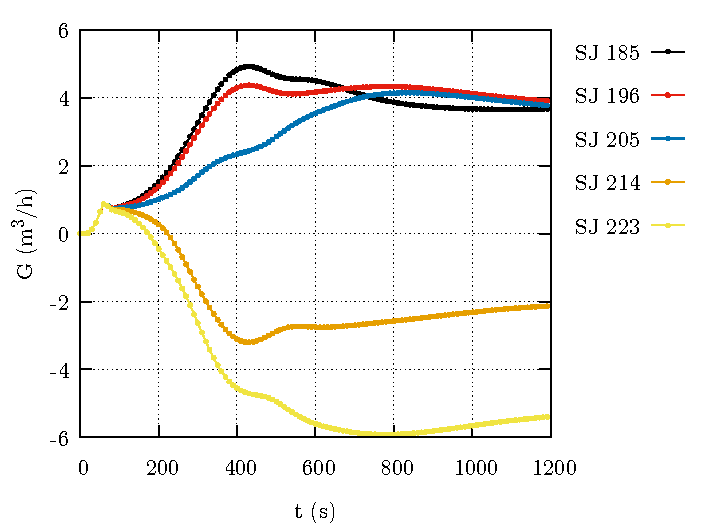
\includegraphics[width=\textwidth, trim={0cm 0cm 0cm 0cm}, clip]{./05_TH_model_VR_1/grafy/G_time_nod_03_2.pdf}
		\caption{S3}
		\label{fig:nod_03_mass_flow_rate_horizontal_s3}
	\end{subfigure}%
	\hfill
	\begin{subfigure}{0.5\textwidth}
		\centering
		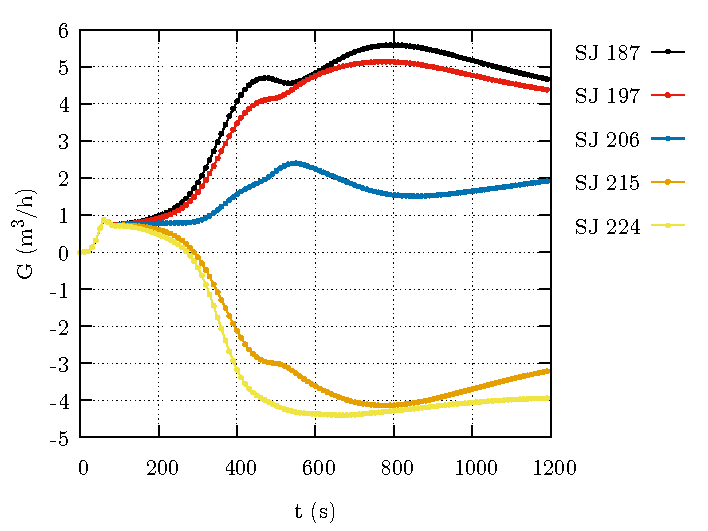
\includegraphics[width=\textwidth, trim={0cm 0cm 0cm 0cm}, clip]{./05_TH_model_VR_1/grafy/G_time_nod_03_3.pdf}
		\caption{S4}
		\label{fig:nod_03_mass_flow_rate_horizontal_s4}
	\end{subfigure}%
	\caption{Průtok skrze jednotlivé SJ (S3 a S4) - model NOD03.}
\end{figure}
V obrázku \ref{fig:nod_03_temp_pipe_40} jsou vykresleny teploty chladiva v jednotlivých nódech trubky 40. Na rozdíl od celkového průtoku je časový vývoj teplot analogický spíše referenčnímu modelu. 
  \begin{figure}[H]
 	\centering
 	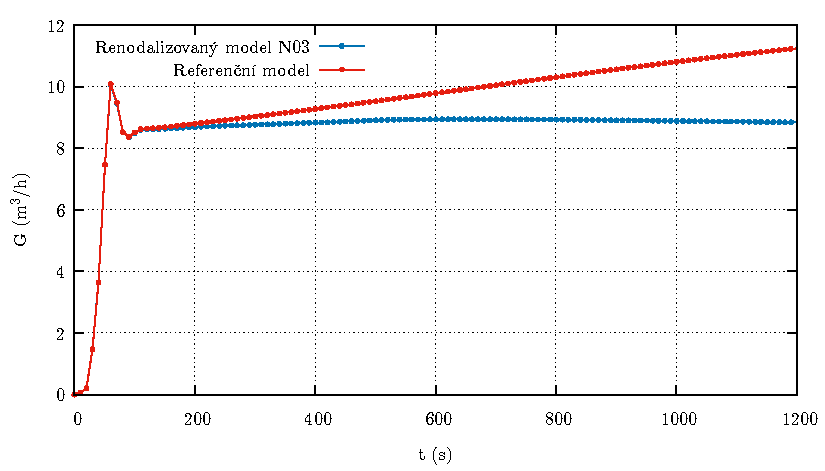
\includegraphics[width=0.8\textwidth]{./05_TH_model_VR_1/grafy/nod_03_mass_flow_rate_vertical.pdf}
 	\caption{Průtok skrze AZ reaktoru VR-1 - referenční a renodalizovaný model NOD03. }
 	\label{fig:nod_03_mass_flow_rate_vertical}
 \end{figure}
% \begin{figure}[H]
% 	\centering
% 	\includegraphics[width=0.8\textwidth]{./05_TH_model_VR_1/grafy/G_time_.pdf}
% 	\caption{Průtok skrze trubky 170 - 174 (viz obr. \ref{fig:nod_01}) - renodalizovaný model NOD01.}
% 	\label{fig:nod_03_mass_flow_rate_horizontal}
% \end{figure}
 \begin{figure}[H]
 	\centering
 	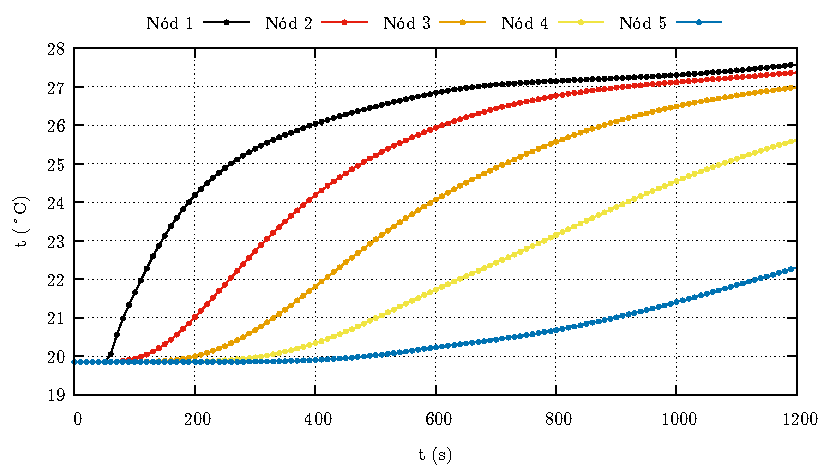
\includegraphics[width=0.8\textwidth]{./05_TH_model_VR_1/grafy/t_nod_03.pdf}
 	\caption{Teplotní vývoj v trubce 40 - model NOD03.}
 	\label{fig:nod_03_temp_pipe_40}
 \end{figure}
% \begin{figure}[H]
% 	\centering
% 	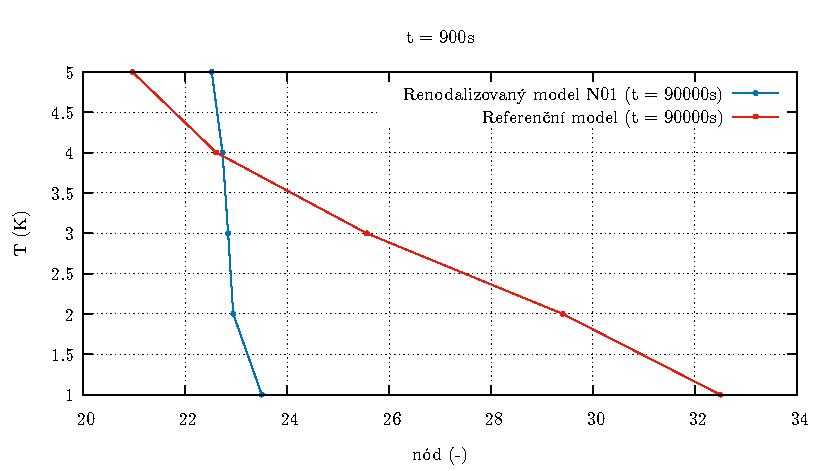
\includegraphics[width=0.8\textwidth]{./05_TH_model_VR_1/grafy/nod_01_900.pdf}
% 	\caption{Distribuce teplot v trubce 40 v čase 900 s.}
% 	\label{fig:nod_01_temp_distribution}
% \end{figure}
% 
 \section{Model NOD04}
 \label{sec:nod_04}
Poslední a nejkomplexnější varianta termohydraulického modelu VR-1 je modifikace modelu NOD03, která částečně vychází z práce \cite{CAPABILITY2017RELAP}. Výsledky získané pro model NOD03 naznačují, že nedochází k ustálení průtoku chladiva skrze jednotlivé skupiny spojovacích jednotek S1 až S6 (více na Obr. \ref{fig:g_time_nod_03_0_prilohy} až \ref{fig:g_time_nod_03_5_prilohy} v příloze). Důvodem fyzikálně neodpovídajících výsledků je nedostatečně propojená vodní hladina s trubkami horizontálního obtoku. Například kapalina v nódu 5 trubky 231 by musela projít minimálně dalšími 11 komponentami než by dorazila do TDV 50 viz obr. \ref{fig:nod_03}. Proto byla do modelu přidána vícenásobná spojovací jednotka (BRANCH) 233 a kontrolní objem 232, které propojují vodní hladinu se všemi skupinami S1 až S6. 
  \begin{figure}[H]
	\centering
\includegraphics[width=0.8\textwidth, trim={7.5cm 243cm 155cm 0cm}, clip]{./07_prilohy/recirkulace/nod_04_recirculation.pdf}
	\caption{Nodalizace horizontálního obtoku - model NOD04}
	\label{fig:nod_04}
\end{figure}
 \subsection{Výsledky}
Na obrázku \ref{fig:nod_04_mass_flow_rate_vertical} je zobrazen celkový průtok chladiva skrze AZ pro referenční model a modely NOD01, NOD03 a NOD04. V případě modelu NOD04 je celkový průtok téměř shodný s modelem NOD03. Dochází však k drastické změně směru proudění ve všech skupinách spojovacích jednotek (SJ), jak je vidět na obrázcích \ref{fig:nod_03} a \ref{fig:nod_04}. Díky odlišné konstrukci vodní hladiny dochází k relativnímu ustálení průtoku v čase okolo 800 s, jak je patrné z obr. \ref{fig:nod_04_mass_flow_rate_horizontal_s3} a \ref{fig:nod_04_mass_flow_rate_horizontal_s4}. Průtok skrze ostatní skupiny je uveden v příloze na obr. \ref{fig:g_time_nod_04_0_prilohy} až \ref{fig:g_time_nod_04_5_prilohy}.
\begin{figure}[H]
	\centering
	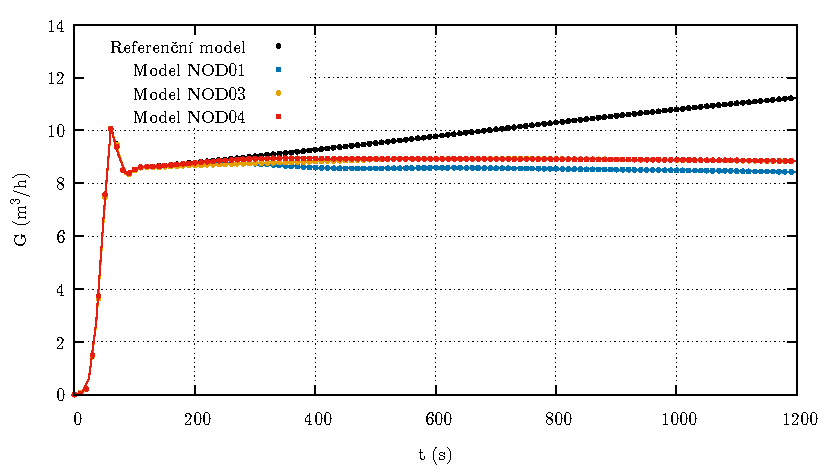
\includegraphics[width=0.8\textwidth]{./05_TH_model_VR_1/grafy/nod_04_mass_flow_rate_vertical.pdf}
	\caption{Průtok skrze AZ reaktoru VR-1 - Referenční model a renodalizovaný model NOD01, NOD03 a NOD04.}
	\label{fig:nod_04_mass_flow_rate_vertical}
\end{figure}
\begin{figure}[H]
	\centering
	\begin{subfigure}{0.5\textwidth}
		\centering
		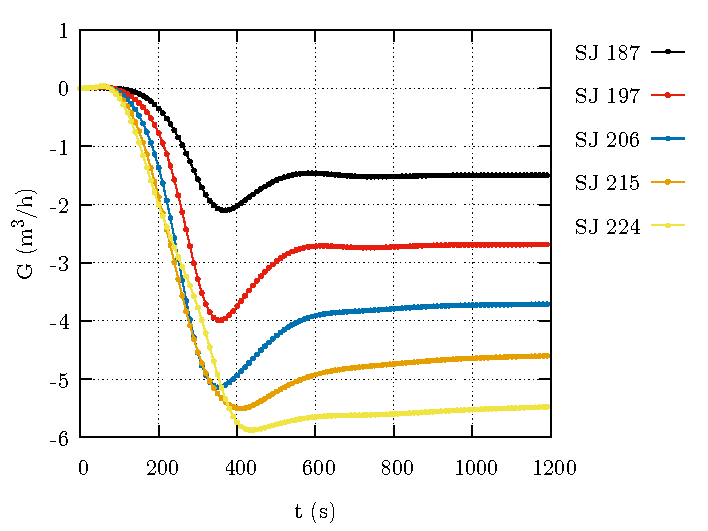
\includegraphics[width=\textwidth, trim={0cm 0cm 0cm 0cm}, clip]{./05_TH_model_VR_1/grafy/G_time_nod_04_2.pdf}
		\caption{S3}
		\label{fig:nod_04_mass_flow_rate_horizontal_s3}
	\end{subfigure}%
	\hfill
	\begin{subfigure}{0.5\textwidth}
		\centering
		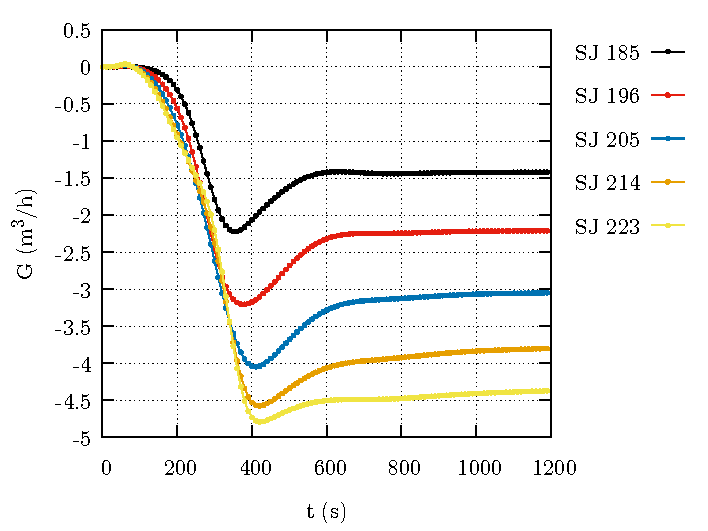
\includegraphics[width=\textwidth, trim={0cm 0cm 0cm 0cm}, clip]{./05_TH_model_VR_1/grafy/G_time_nod_04_3.pdf}
		\caption{S4}
		\label{fig:nod_04_mass_flow_rate_horizontal_s4}
	\end{subfigure}%
	\caption{Průtok skrze jednotlivé SJ (S3 a S4) - model NOD04.}
\end{figure}
 \begin{figure}[H]
 	\centering
 	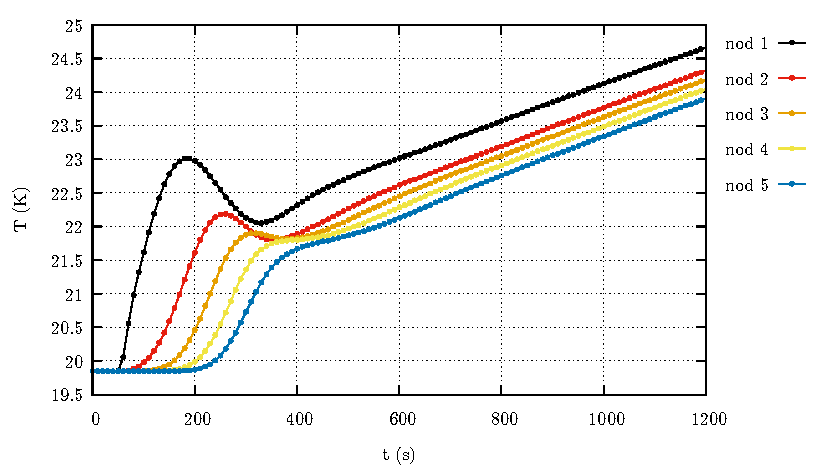
\includegraphics[width=0.8\textwidth]{./05_TH_model_VR_1/grafy/tempf_nod_04_1.pdf}
 	\caption{Teplotní vývoj v trubce 40 - model NOD04.}
 \end{figure}
 
 
 
 
 